% CREATED BY DAVID FRISK, 2015
\chapter{Methods}



There are different ways to find or generate geodesic on a surface. In this chapter two possible ways will be described. The two different approaches differs in the sense of its initial condition. Either you can generate the geodesics in a form finding process or you can start from an already defined surface.



\section{Compatibility of Differential geometry and Membrane theory}

With the theory in mind from sections regarding differential geometry and 
Assuming we have know loadings of the membrane we have 9 components that are unknown:

\[ 
\left \{
  \begin{tabular}{ccc}
  $a_{11}$  & $a_{12} =a_{21} $ & $a_{22}$ \\
 $b_{11}$  & $b_{12} =b_{21} $ & $b_{22}$\\
  $n_{11}$  & $n_{12} =n_{21} $ & $n_{22}$ 
  \end{tabular}
\right \}
\]

\vspace{5mm}
Obviously that means we need 9 equations to solve 9 unknown components. Gauss and Codazzi proved that the first and second fundamental form is indeed connected. Green and Zerna shows through the equilibrium connects the first and second fundamental form to the stress components. 
\vspace{5mm}

Three equations arise from the equilibrium equations.

$$n^{\alpha \beta}b_{\alpha \beta} + p = 0$$
$$n^{\alpha \beta}|_\alpha + p^\beta = 0$$

Three equations arise from equations of Gauss(Theorema egregium) and Codazzi.


$$ b_{11},_2 - b_{12},_1 = b_{11} \Gamma^1_{12} + b_{12}(\Gamma^2_{12} - \Gamma^1_{11}) - b_{22}\Gamma^2_{11} $$
$$   b_{12},_2 - b_{22},_1 = b_{11} \Gamma^1_{22} + b_{12}(\Gamma^2_{22} - \Gamma^1_{12}) - b_{22}\Gamma^2_{12} $$
$$  K= \frac{b_{11}b_{22}-b^2_{12}}{a}$$

That is in total 6 equations so it is still three unknown. It is possible to impose more known conditions than the loads alone. Two examples of these are
\vspace{5mm}
\begin{enumerate}
\item \textit{Geodesic coordinates}, $a_{22} = L^2 = const, a_{12}=0$
\begin{figure}[H]
\centering
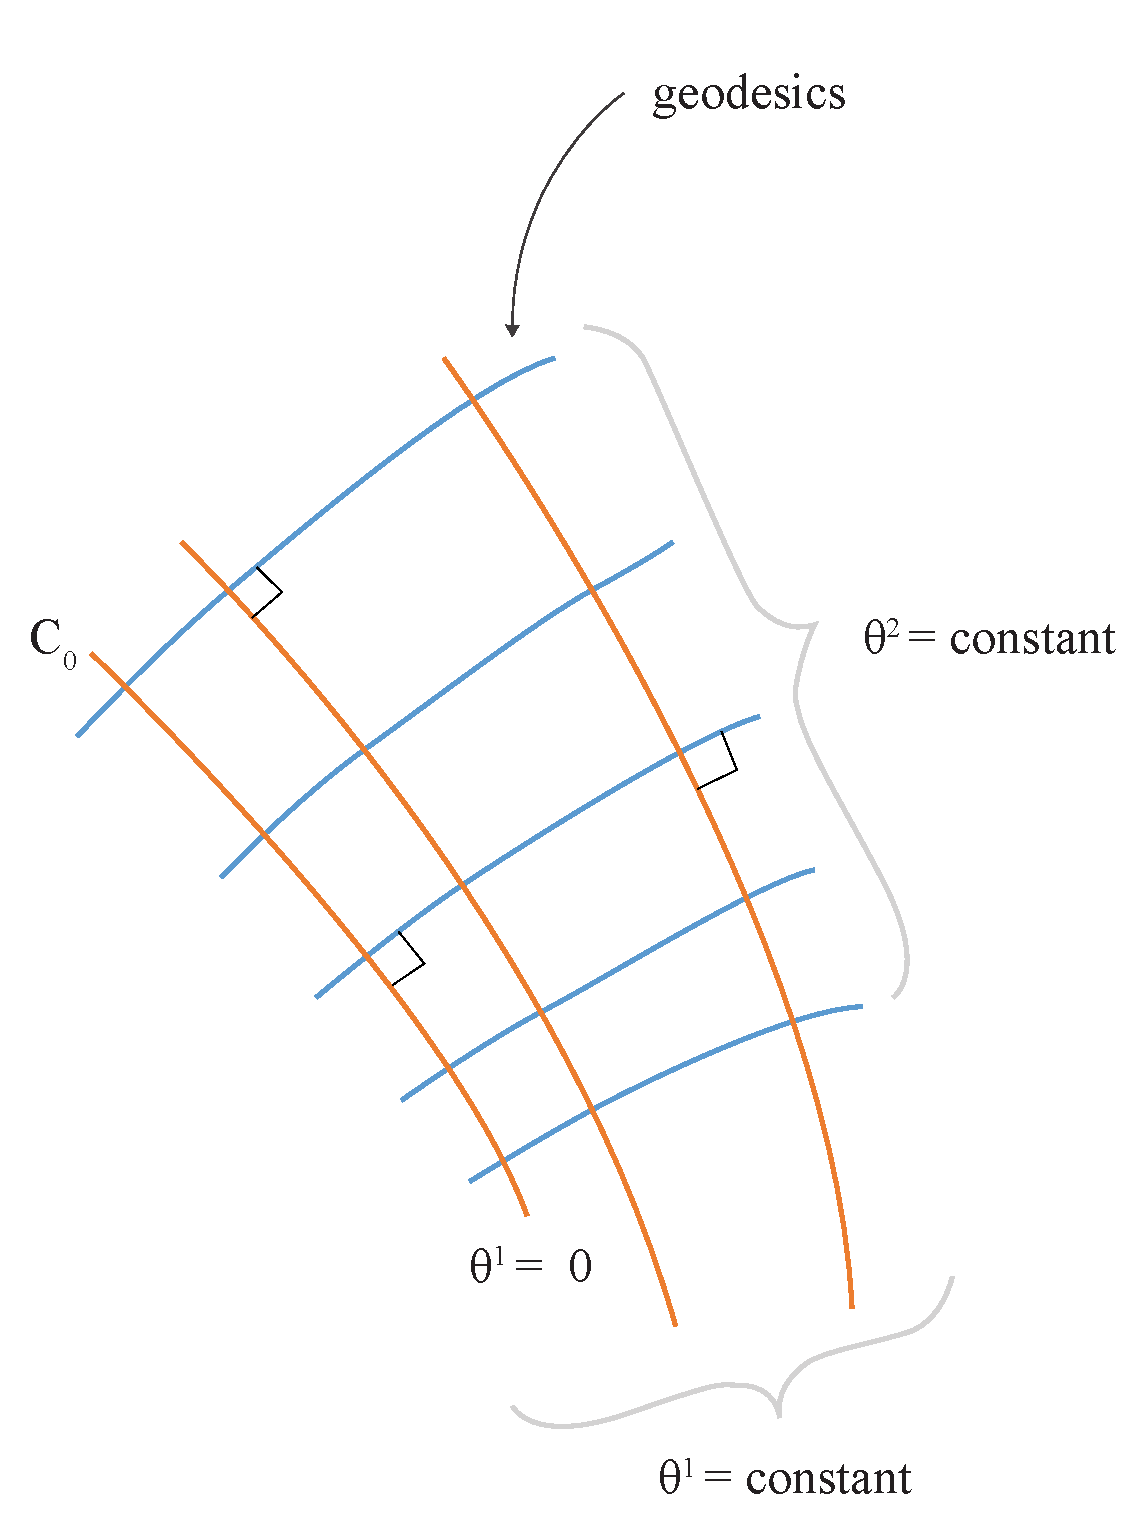
\includegraphics[height=0.7\linewidth ]{figure/Theory/geodesicCoordRe.pdf}
\end{figure}
\item \textit{Equal mesh net coordinates}, $a_{11}= a_{22} = L^2, n_{12}=0$ 
\begin{figure}[H]
\centering
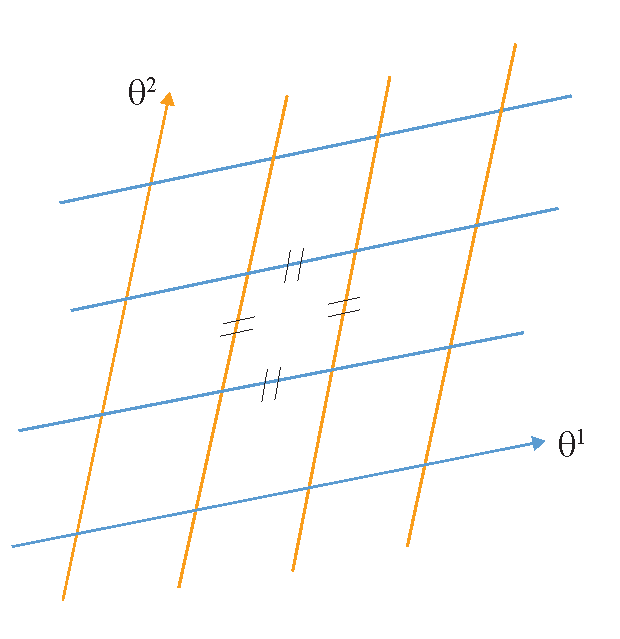
\includegraphics[height=0.4\linewidth ]{figure/Theory/equalMeshFrei.pdf}
\end{figure}
\end{enumerate}

In Williams case it is for membrane structures where he uses 
\section{Separated form and geodesic generation}

This method as it states separate the form generation and the geodesic pattern generation. Therefore it gives more freedom in the sense that the form-generation can be focused on spatial and structural requirements. The method can be divided into three different stages.

\begin{enumerate}
\item Generate a form that satisfies equilibrium for masonry structures
\item Generate geodesics on that surface
\item Generate the orthogonal trajectories that cuts the geodesics in equal length curves. 
\end{enumerate}

\subsection{Form finding}
For this purpose it is only interesting to use numerical form-finding methods. It should be possible to choose whichever that pleases you where you can apply vertical loads for self-weight. For masonry structures it is important though that all forces and stresses acts in compression. The most suitable method for masonry structures is the TNA but it not implemented in a parametric environment, so far, so in this case traditional FD or DR method will be used.
\subsection{Generation of geodesics and orthogonal trajectories}

It is possible to generate geodesics on a surface using for instance a DR or PS solver. The main idea is to model the geodesics as a set of springs that can move on the surface only. The springs should only be loaded with a pre-tensional force. The goal is to reduce the force component in the geodesic direction,i.e the geodesic curvature. It is possible to check this geodesic condition geometrically for each point, or node in this case. Taking the cross product of the vectors in the same direction of the springs it should be perpendicular to the normal in the node point. 



\begin{figure}[H]
\centering
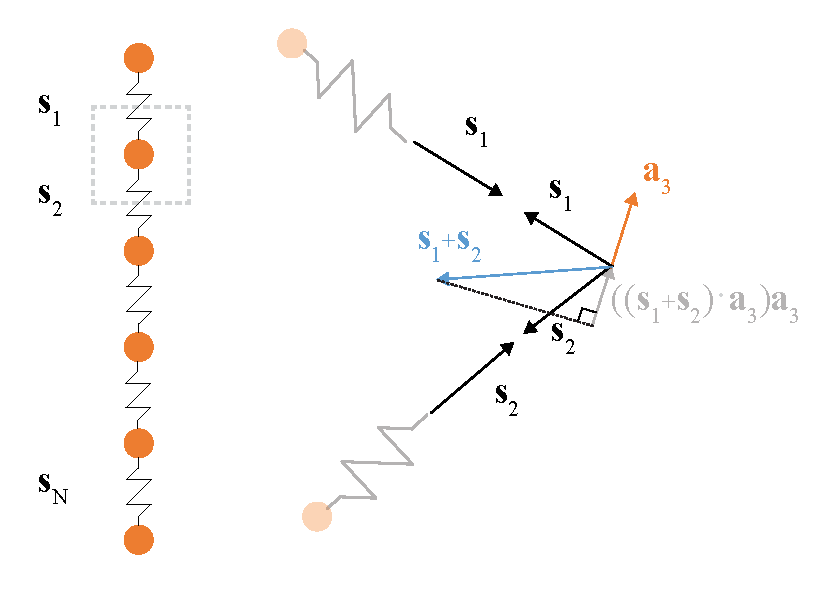
\includegraphics[width = 0.6\linewidth ]{figure/Method/GeodesicDyn.pdf}
\centering
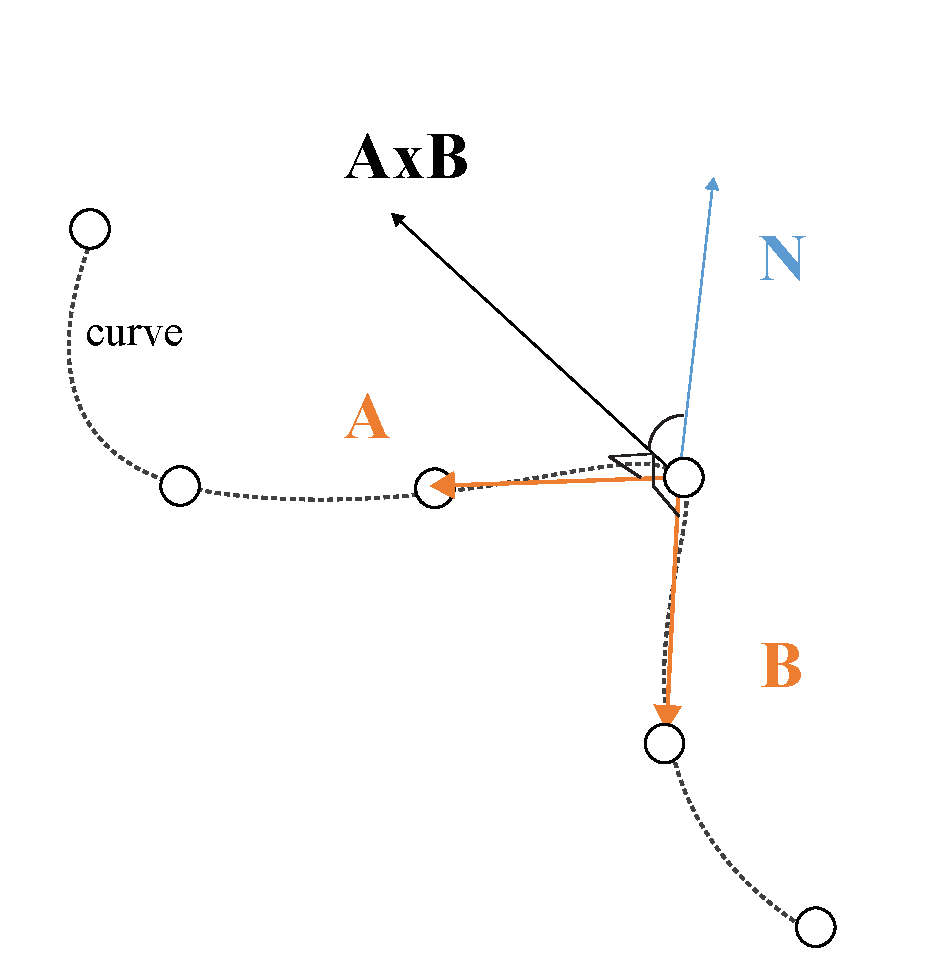
\includegraphics[width = 0.35\linewidth ]{figure/Method/ChreckDR3.pdf}
\caption{http://web.mit.edu/hyperbook/Patrikalakis-Maekawa-Cho/node29.html}
\end{figure}


\vspace{5mm}


\begin{enumerate}
\item Decide the end points of the geodesics on the surface.
\item Generate an initial curve that lies on the surface
\item Discretize  the curve into segments, small enough to resemble the curve properties, of the same length. This segments will be the springs in the DR or PS algorithm.
\item Apply the same pretension in all elements and ensure that the nodes move along the surface, this can be done by either a force or just moving the point to surface in each iteration. 
\item Start the solver, and for each iteration check the geodesic requirement for each point, or node. When all nodes are geodesic points then solution has converged and the iterations end.
\end{enumerate}



\section{Simultaneous form and geodesic generation}

In the paper Air supported structure the state of art Williams present a method to combine form finding with the generation of cutting patterns for air-supported tensile structures, i.e finding shapes of equilibrium that applies geodesic coordinates where one of the set curves are geodesics. The fundamental requirement, Willams states, is that under internal pressure the principal stress in the membrane should be tensile. Therefore this is not directly applicable to masonry structures.

\vspace{5mm}
\begin{enumerate}
\item To simultaneously find a form in equilibrium and geodesic lines on the surface
\item To have a stress distribution in the surface under inflation pressure such that the principal stress directions coincide with the warp and weft directions of the fabric. The simples stress distribution is the uniform(or soap film) but many others are possible.
\end{enumerate}
\vspace{5mm}
The nodes can move in three different directions.
\begin{enumerate}
\item Normal to the surface according to the equilibrium requirements

\item In the plane of the surface perpendicular to the geodesics to make (angle1 + angle2 + angle3 = angle4 + angle5 + angle6).
\begin{figure}[H]
\centering
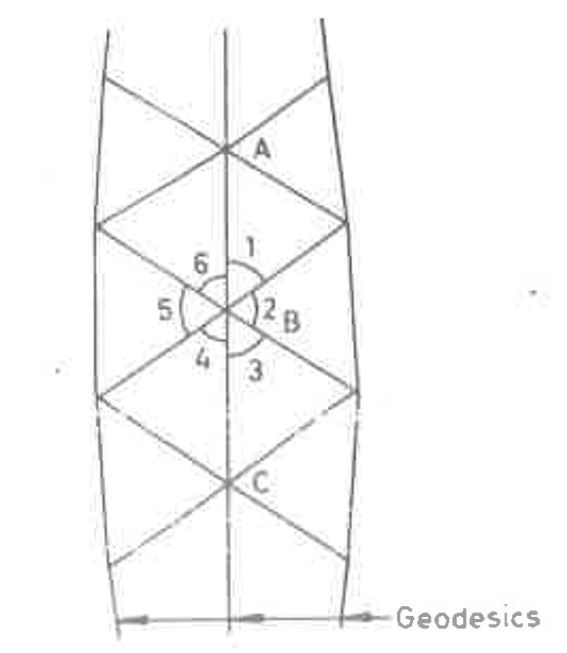
\includegraphics[height = 0.4\linewidth ]{figure/Method/method2A.JPG}
\caption{}
\end{figure}
\item In the plane of the surface parallel to the geodesics to make the length AB equal to BC
\begin{figure}[H]
\centering
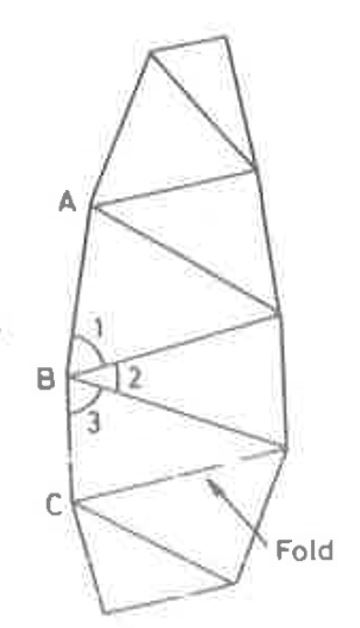
\includegraphics[height = 0.4\linewidth ]{figure/Method/method2B.JPG}
\caption{}
\end{figure}
\end{enumerate}